%-------------------------------------------
% YOUR THESIS
%-------------------------------------------

\documentclass[12pt,titlepage, dvipsnames]{article}

%-------------------------------------------
%SETTINGS
%DO NOT TOUCH EXCEPT YOU REALLY KNOW WHAT YOU ARE DOING!
%-------------------------------------------

\usepackage[style=apa, natbib=true]{biblatex}
\bibliography{04_bibliography.bib}
\usepackage{lipsum}
\usepackage[english]{babel}
\usepackage[utf8]{inputenc}
\usepackage[a4paper,lmargin={2.5cm},rmargin={2.5cm},tmargin={2.5cm},bmargin =
{2.5cm}]{geometry}
\usepackage{amssymb}
\usepackage[bottom, hang]{footmisc} %makes footnotes stick to the bottom page
\setlength{\footnotemargin}{1em}
\setlength{\footnotesep}{0.4cm}
\interfootnotelinepenalty=10000 %makes latex less likely to pagebreak a footnote
\usepackage{tablefootnote}
%\renewcommand{\footnotesize}{\small} %change \small set the desired size of your footnotes
\usepackage[dvipsnames, table]{xcolor}
\usepackage{csquotes}
\usepackage{amsthm}
\usepackage{graphicx}
\usepackage{enumitem}
\usepackage{booktabs}
\usepackage{soul}
\usepackage{caption}
\usepackage{subcaption}
\usepackage{array,multirow}
\usepackage{pgfplots}
\usepackage{textcomp}
\newcounter{savepage}
\setlength{\parindent}{0pt} %the indentation when you start a new paragraph
\setlength{\parskip}{1.3em} %the space between each paragraph
\usepackage{amsmath}
\numberwithin{equation}{subsection}
\usepackage{mathtools}
\usepackage{tikz}
\usepackage{float}
\usepackage{tabularx}
\usepackage{multicol}
\usepackage{dcolumn}
\usepackage[export]{adjustbox}
\usepackage{tocloft} %advanced TOC, LOF and LOT options
\newcommand\tab[1][1cm]{\hspace*{#1}}
\renewcommand{\cftfigpresnum}{Fig. }
\renewcommand{\cfttabpresnum}{Tab. }
\renewcommand{\cftfigaftersnum}{:}
\renewcommand{\cfttabaftersnum}{:}
\setlength{\cftfignumwidth}{2cm}
\setlength{\cfttabnumwidth}{2cm}
\setlength{\cftfigindent}{0cm}
\setlength{\cfttabindent}{0cm}
\usetikzlibrary{decorations.pathreplacing}
\usepackage[super]{nth}
\usepackage{fancyhdr}
\setlength{\headheight}{14.5pt}
\pagestyle{fancy}
\fancyhf{}
\rhead{\thepage}
\lhead{\nouppercase\leftmark}
\usepackage{pdfpages} %insert pdf pages
\usepackage{pdflscape}
\usepackage{longtable} %edit longtable format and row color
\definecolor{lightgray}{gray}{0.9}
\let\oldlongtable\longtable
\let\endoldlongtable\endlongtable
\renewenvironment{longtable}{\rowcolors{2}{white}{lightgray}\oldlongtable} {
\endoldlongtable}

%\usepackage[hyphens]{url}
\urlstyle{same}
\usepackage{setspace}
\onehalfspacing
\usepackage[hidelinks]{hyperref}
\renewcommand{\UrlBreaks}
{\do\a\do\b\do\c\do\d\do\e\do\f\do\g\do\h\do\i\do\j\do\k\do\l\do\m\do\m\do\n\do\o\do\p\do\q\do\r\do\s\do\t\do\u\do\v\do\w\do\x\do\y\do\z\do\1\do\2\do\3\do\4\do\5\do\6\do\7\do\8\do\9\do\.\do\_\do\?\do\!\do\-\do\&}

\usepackage[automake,style=super,nopostdot,nonumberlist]{glossaries}
%if you want to display the page number, delete nonumberlist
\makeglossaries
\renewcommand{\glsnamefont}[1]{\textbf{#1}}
\renewcommand*{\glsgroupskip}{} %activate for smaller linespacing



\begin{document}

%-------------------------------------------
% TITLEPAGE
%-------------------------------------------

\begin{titlepage}
  \centering
  
\includegraphics[width=8cm]{images/yourlogo.png}\par\vspace{1cm}
  \linespread{1}\Large{\scshape Your Institute\par}
  \vspace{1.5cm}
  {\scshape\Large\bfseries Bachelor Thesis\par}
  {\huge\bfseries The Little Prince Template \par
    \Large\bfseries *insert subtitle here*\par}
  \vspace{1.5cm}
  \linespread{0.75}\Large{Your Name\par Your Number\par Street\par ZIP Code}
  \vfill
  \linespread{0.75}\large{Submitted to:\par
    Prof. Test}
  \vfill
  % Bottom of the page
  {\large 23.02.2042\par}
\end{titlepage}

%-------------------------------------------
% ABSTRACT
%-------------------------------------------

\pagenumbering{roman}
\section*{Abstract}
\lipsum[1] %write you abstract here

\phantomsection %command is necessary for hyperref to jump to the correct page
\addcontentsline{toc}{section}{Abstract}

%-------------------------------------------
% TOC, FIGURES, TABELES, ABBREVIATIONS
%-------------------------------------------

\newpage
\phantomsection
\renewcommand{\contentsname}{Table of Contents}
\addcontentsline{toc}{section}{Table of Contents}
\tableofcontents\thispagestyle{fancy}

\newpage
\listoffigures\thispagestyle{fancy}
\phantomsection
\addcontentsline{toc}{section}{List of Figures}

\newpage
\listoftables\thispagestyle{fancy}
\phantomsection
\addcontentsline{toc}{section}{List of Tables}

\newpage
%-------------------------------------------
%ABBREVIATIONS
%-------------------------------------------

%basic syntax (automatically alphabetically ordered in compiled file)
%\newglossaryentry{⟨label⟩}{name={⟨key⟩}, description={⟨value⟩}}


\newglossaryentry{ann}{name={ANN},description={Artificial Neural Network}}

\printglossary[title = List of Abbreviations]\thispagestyle{fancy}
\phantomsection
\addcontentsline{toc}{section}{List of Abbreviations}

\newpage
\setcounter{savepage}{\arabic{page}}
\pagenumbering{arabic}

%-------------------------------------------
% MAIN BODY
%-------------------------------------------

\section{Introduction}
  \label{sec:Intro}
{\centering
``And now here is my secret, a very simple secret: It is only with the heart that one can see rightly; what is essential is invisible to the eye."\footnote{The Little Prince (2018). Personal communication.}	\par
}

\lipsum[1-3]

\newpage

\section{Chapter1}
	\label{sec:chapter1}

	Some references using \LaTeX

	\citet{de1998little}

	\citet[p.~34]{de1998little}

	\citep{de1998little}

	\citep[p.~34]{de1998little}

	\citep{de1998little,bieger2013}

	(\citealp[p.~3]{de1998little}; \citealp[p.~5]{bieger2013})

	\citep[e.g.][p.~34]{de1998little}

	\textbf{How to use Glossary/Abbreviation function}

\gls{ann}, as the name already reveals, are computational networks that are able to solve complex, nonlinear mathematical problems.

\subsection{Equations}
	\label{subsec:equ}


	\begin{equation}
	\mathrm C( S, t)= \mathrm N(\mathrm d_1)\mathrm S - \mathrm N(\mathrm d_2) \mathrm K \mathrm e^{-rt}
	\label{eq:1}
	\end{equation}

	\begin{equation}
	\mathrm d_2= \mathrm d_1 - \sigma \sqrt{\mathrm t}
	\label{eq:3}
	\end{equation}

	\newpage

\section{Chapter2}
		\label{sec:chapter2}

	\lipsum[1]
	\begin{figure} [H]
	 \centering
	  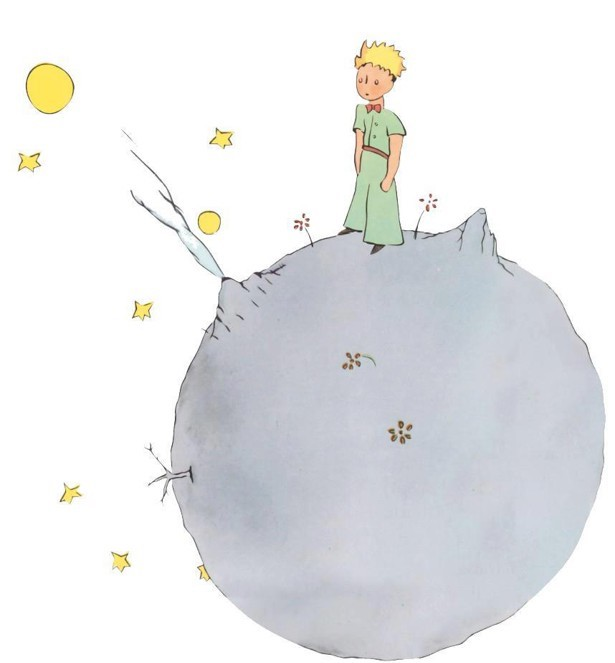
\includegraphics[width=0.75\textwidth]{images/princeplanet.jpg}
		\caption[The little prince on planet b612]{\centering \textit{The little prince on planet b612}}
	  \label{fig:1}
	\end{figure}
\newpage


%-------------------------------------------
% REFERENCES, APPENDIX, DECLARATION
%-------------------------------------------

%-------------------------------------------
%REFERENCES
%DO NOT TOUCH EXCEPT YOU REALLY KNOW WHAT YOU ARE DOING!
%-------------------------------------------
\newpage
%\section*{References}
\phantomsection
\addcontentsline{toc}{section}{References}
\setlength\bibitemsep{12pt}   % length between two different entries
\printbibliography


%if not working, try to change bibliography engine in your settings of your app/machine
%-------------------------------------------
%APPENDIX
%DO NOT TOUCH EXCEPT YOU REALLY KNOW WHAT YOU ARE DOING!
%-------------------------------------------
\newpage
\begin{appendix}
%\appendix
\renewcommand{\thesection}{\Alph{section}}
\renewcommand{\appendixname}{Appendix}
\renewcommand{\thesubsection}{\thesection.\arabic{subsection}}
\renewcommand\thefigure{\thesection.\arabic{figure}}
\renewcommand\thetable{\thesection.\arabic{table}}
\setcounter{table}{0}
\setcounter{figure}{0}

\begin{landscape}

\section{Appendix}
\subsection{Sample Longtable Format}
\label{app:sample}

\renewcommand{\arraystretch}{1.2}
\begin{longtable}{
>{\centering\arraybackslash}m{1cm} %id
>{\centering\arraybackslash}m{2.5cm} %Source
>{\centering\arraybackslash}m{4cm} %Autors
>{\centering\arraybackslash}m{1.8cm} %year
>{\centering\arraybackslash}m{13cm} % Title
}

 %header
 \rowcolor[rgb]{ .149,  .149,  .149}
 \textcolor[rgb]{ 1,  1,  1}{\textbf{ID}} & 
 \textcolor[rgb]{ 1,  1,  1}{\textbf{Source}} & 
 \textcolor[rgb]{ 1,  1,  1}{\textbf{Authors}} & 
 \textcolor[rgb]{ 1,  1,  1}{\textbf{Year}} &
 \textcolor[rgb]{ 1,  1,  1}{\textbf{Title}} \\
%content


001   & arXiv.org & Bornas and Mateos & 2019  & A Character-Level Approach to the Text Normalization Problem Based on a New Causal Encoder \\
002   & arXiv.org & Kalyan and Sangeetha & 2019  & SECNLP: A Survey of Embeddings in Clinical Natural Language Processing \\
003   & arXiv.org & Zhang et al. & 2019  & Multiresolution Graph Attention Networks for Relevance Matching \\
004   & arXiv.org & Monti et al. & 2019  & Fake News Detection on Social Media using Geometric Deep Learning \\
005   & arXiv.org & Si et al. & 2019  & Enhancing Clinical Concept Extraction with Contextual Embedding \\
006   & arXiv.org & Vo et al. & 2019  & Combination of Domain Knowledge and Deep Learning for Sentiment Analysis of Short and Informal Messages on Social Media \\
007   & arXiv.org & Vidya et al. & 2019  & A Deep Learning Approach for Similar Languages, Varieties and Dialects \\
008   & arXiv.org & Eger et al. & 2019  & Is it Time to Swish? Comparing Deep Learning Activation Functions Across NLP tasks \\
009   & arXiv.org & Wolk et al. & 2019  & Deep learning and sub-word-unit approach in written art generation. \\

 	    \bottomrule
\rowcolor{white} 	    
  \caption[Table of Sample (cross-references)]{\textit{Complete table of samples obtained from cross-references. (own table)}}
 \end{longtable}
  \label{app:crossrefsample}
  
\end{landscape}



\end{appendix}

%-------------------------------------------
%DECLARATION
%-------------------------------------------
\newpage
\thispagestyle{empty}

\section*{Declaration of Authorship}
“I hereby declare
\begin{itemize}
	\item that I have written this thesis without any help from others and without the use of documents and aids other than those stated above;

	\item that I have mentioned all the sources used and that I have cited them correctly according to established academic citation rules;

	\item that I have acquired any immaterial rights to materials I may have used such as images or graphs, or that I have produced such materials myself;

	\item that the topic or parts of it are not already the object of any work or examination of another course unless this has been explicitly agreed on with the faculty member in advance and is referred to in the thesis;

	\item that I will not pass on copies of this work to third parties or publish them without the University’s written consent if a direct connection can be established with the  or its faculty members;

	\item that I am aware that my work can be electronically checked for plagiarism and that I hereby grant the copyright in accordance with the Examination Regulations in so far as this is required for administrative action;

	\item that I am aware that the University will prosecute any infringement of this declaration of authorship and, in particular, the employment of a ghostwriter, and that any such infringement may result in disciplinary and criminal consequences which may result in my expulsion from the University or my being stripped of my degree.”


\end{itemize}

\vspace{1cm}

\begin{minipage}{6.5cm}
\dotfill
\end{minipage} %\newline
\newline
St.Gallen, \today

\scriptsize{By submitting this academic term paper, I confirm through my conclusive action that I am submitting the Declaration of Authorship, that I have read and understood it, and that it is true.}


\end{document}
